\section{General Scheme}\label{sec:general-scheme}

The field of anomaly detection in CPS and IoT environments encompasses a wide range of methodologies, from machine learning and deep learning approaches to invariant-based techniques and other innovative strategies. Despite the diversity of these methods, they generally adhere to a common framework that includes several key steps:
\begin{enumerate}
    \item \textbf{Data Collection:} Gathering relevant data from various sensors, actuators, and network components of the CPS or IoT environment. This involves collecting both normal operational data and, when possible, data representing known anomalies or attack scenarios.
    
    \item \textbf{Data Preprocessing:} Cleaning, normalizing, and transforming the collected data to make it suitable for analysis. This step may involve handling missing values, removing noise, scaling features, and applying dimensionality reduction techniques.
    
    \item \textbf{Feature Extraction and Selection:} Identifying and selecting the most relevant features that effectively capture the system's behavior and are indicative of potential anomalies. This may involve time-series analysis, statistical methods, or domain-specific knowledge.
    
    \item \textbf{Model Training and Baseline Establishment:} Developing and training the chosen anomaly detection model using the preprocessed data. This step involves establishing a baseline of normal system behavior, which serves as a reference point for detecting deviations.
    
    \item \textbf{Real-time Monitoring and Anomaly Detection:} Continuously analyzing incoming data streams in real-time, comparing them against the established baseline or model predictions. When significant deviations are detected, the system flags these as potential anomalies for further investigation or immediate action.
\end{enumerate}

Figures \ref{fig:general-view} and \ref{fig:general-steps} illustrate the process of anomaly detection in CPS. Figure \ref{fig:general-view} provides a general overview, highlighting how normal and abnormal behaviors are identified and alerts are triggered when an attack or failure is detected. Figure \ref{fig:general-steps} elaborates on the workflow for anomaly detection, detailing steps such as data collection, preprocessing, feature extraction, model training, and real-time monitoring.

While the specific implementation of these steps varies across different methodologies, this general framework provides a foundation for effective anomaly detection. Machine learning and deep learning approaches excel in learning complex patterns from large datasets, while invariant-based methods offer interpretable and physically meaningful constraints. Other methodologies, such as bio-inspired algorithms, timing-based detection, and integrated cyber-physical approaches, provide unique perspectives on identifying anomalies in these complex systems.

\subsection{Choosing Anomaly Detection Approaches}

The choice of approach often depends on the specific requirements of the CPS or IoT environment, including factors such as the availability of labeled data, the need for real-time detection, the complexity of the system, and the types of anomalies being targeted. As CPS continue to grow in complexity and face evolving threats, the field of anomaly detection is likely to see further innovations. Future research may focus on integrating multiple approaches to create more robust, adaptive, and comprehensive anomaly detection systems capable of addressing the diverse challenges in securing critical infrastructure and IoT networks.


As shown in the image\ref{fig:example-image}, we categorized anomaly detection methods into seven sections: Machine Learning, Deep Learning, Machine and Deep Learning, Mathematics, Hybrid, Invariant, and Hybrid Methods. While the number of articles we reviewed varies across different years, we focused on selecting the most important papers, regardless of the approach. The graph highlights a noticeable trend over time, particularly after 2018, there has been a growing emphasis on Machine Learning and Deep Learning approaches.

\begin{figure}[h]
    \centering
    \includegraphics[width=0.5\textwidth]{images/approach.png}
    \caption{Categorizing different anomaly detection approaches over time}
    \label{fig:example-image}
\end{figure}




\begin{comment}
\begin{figure}[h]
\centering
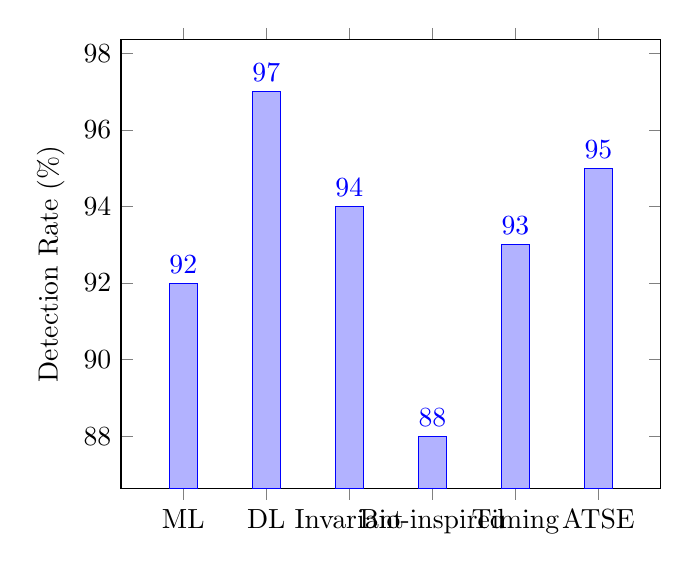
\begin{tikzpicture}
\begin{axis}[
    ybar,
    enlargelimits=0.15,
    legend style={at={(0.5,-0.15)},
      anchor=north,legend columns=-1},
    ylabel={Detection Rate (\%)},
    symbolic x coords={ML, DL, Invariant, Bio-inspired, Timing, ATSE},
    xtick=data,
    nodes near coords,
    nodes near coords align={vertical},
    ]
\addplot coordinates {(ML,92) (DL,97) (Invariant,94) (Bio-inspired,88) (Timing,93) (ATSE,95)};
\end{axis}
\end{tikzpicture}
\caption{Comparison of Detection Rates for Different Anomaly Detection Methods}
\label{fig:detection_rates}
\end{figure}

\begin{table}[h]
\centering
\caption{Applicability of Methods to Different CPS Domains}
\label{tab:applicability}
\begin{tabular}{|l|c|c|c|c|}
\hline
\textbf{Method} & \textbf{Smart Grid} & \textbf{Industrial IoT} & \textbf{Smart Cities} & \textbf{Healthcare CPS} \\
\hline
Machine Learning & \checkmark & \checkmark & \checkmark & \checkmark \\
Deep Learning & \checkmark & \checkmark & \checkmark & \checkmark \\
Invariant-based & \checkmark & \checkmark & & \checkmark \\
Bio-inspired (iDCA) & & \checkmark & \checkmark & \\
Timing-based & & \checkmark & & \\
ATSE & \checkmark & & & \\
\hline
\end{tabular}
\end{table}



\begin{figure}[h]
\centering
\begin{tikzpicture}
\pie{25/Machine Learning, 30/Deep Learning, 20/Invariant-based, 10/Bio-inspired, 8/Timing-based, 7/ATSE}
\end{tikzpicture}
\caption{Distribution of Research Focus in Anomaly Detection Methods}
\label{fig:research_focus}
\end{figure}

\end{comment}

\begin{comment}
\begin{table*}[h]
\centering
\caption{Comprehensive Comparison of Anomaly Detection Approaches in CPS and IoT}
\label{tab:anomaly_comparison}
\resizebox{\textwidth}{!}{%
\begin{tabular}{|l|c|c|c|c|c|c|}
\hline
\textbf{Approach} & \textbf{Scalability} & \textbf{Interpretability} & \textbf{Adaptability} & \textbf{Data Requirements} & \textbf{Computational Cost} & \textbf{Key Strengths} \\
\hline
Machine Learning & High & Medium & Medium & Medium & Medium & 
\begin{tabular}[c]{@{}c@{}}Effective for structured data; \\ Good for known patterns\end{tabular} \\
\hline
Deep Learning & Medium & Low & High & High & High & 
\begin{tabular}[c]{@{}c@{}}Excellent for complex patterns; \\ Handles high-dimensional data\end{tabular} \\
\hline
Machine Learning and Deep Learning & High & Medium & High & High & Medium-High & 
\begin{tabular}[c]{@{}c@{}}Combines strengths of ML and DL \\ for better performance\end{tabular} \\
\hline
Hybrid & High & Medium & High & Medium & Medium-High & 
\begin{tabular}[c]{@{}c@{}}Versatile and robust; \\ Combines strengths of multiple approaches\end{tabular} \\
\hline
Mathematics & High & High & Low & Medium & Low & 
\begin{tabular}[c]{@{}c@{}}Strong theoretical foundation; \\ Effective for mathematical analysis\end{tabular} \\
\hline
Invariant-based & Medium & High & Low & Low & Low & 
\begin{tabular}[c]{@{}c@{}}Strong theoretical foundation; \\ Effective for systems with clear constraints\end{tabular} \\
\hline
Other & Medium & Medium & Medium & Medium & Medium & 
\begin{tabular}[c]{@{}c@{}}Novel and adaptable; \\ Addresses niche problems effectively\end{tabular} \\
\hline
\end{tabular}%
}
\end{table*}
\end{comment}













\begin{comment}
    

\begin{table*}[h]
\centering
\caption{Comprehensive Comparison of Anomaly Detection Approaches in CPS and IoT}
\label{tab:anomaly_comparison}
\resizebox{\textwidth}{!}{%
\begin{tabularx}{\textwidth}{@{}p{3cm}XXXXXp{4cm}@{}}
\toprule
\textbf{Approach} & \textbf{Scalability} & \textbf{Interpretability} & \textbf{Adaptability} & \textbf{Data Requirements} & \textbf{Computational Cost} & \textbf{Key Strengths} \\
\midrule
Machine Learning & High & Medium & Medium & Medium & Medium & Effective for structured data; good for known patterns. \\
Deep Learning & Medium & Low & High & High & High & Excellent for complex patterns; handles high-dimensional data. \\
Machine Learning and Deep Learning & High & Medium & High & High & Medium-High & Combines strengths of ML and DL for better performance. \\
Hybrid & High & Medium & High & Medium & Medium-High & Versatile and robust; combines strengths of multiple approaches. \\
Mathematics & High & High & Low & Medium & Low & Strong theoretical foundation; effective for mathematical analysis. \\
Invariant-based & Medium & High & Low & Low & Low & Strong theoretical foundation; effective for systems with clear constraints. \\
\bottomrule
\end{tabularx}%
}
\end{table*}
\end{comment}

Table \ref{tab:anomaly_comparison} comprehensive comparison highlights the strengths and weaknesses of various anomaly detection approaches in CPS and IoT, helping identify the most suitable techniques based on specific application requirements.










\begin{comment}
    

\begin{table}[h]
\centering
\caption{Comprehensive Comparison of Anomaly Detection Approaches in CPS and IoT}
\label{tab:anomaly_comparison}
\resizebox{\textwidth}{!}{%
\begin{tabular}{|l|c|c|c|c|c|c|}
\hline
\textbf{Approach} & \textbf{Scalability} & \textbf{Interpretability} & \textbf{Adaptability} & \textbf{Data Requirements} & \textbf{Computational Cost} & \textbf{Key Strengths} \\
\hline
Machine Learning & High & Medium & Medium & Medium & Medium & 
\begin{tabular}[c]{@{}c@{}}Effective for structured data\\ Good for known patterns\end{tabular} \\
\hline
Deep Learning & Medium & Low & High & High & High & 
\begin{tabular}[c]{@{}c@{}}Excellent for complex patterns\\ Handles high-dimensional data\end{tabular} \\
\hline
Hybrid & High & Medium & High & Medium & Medium-High & 
\begin{tabular}[c]{@{}c@{}}Versatile and robust\\ Combines strengths of multiple approaches\end{tabular} \\
\hline
Invariant-based & Medium & High & Low & Low & Low & 
\begin{tabular}[c]{@{}c@{}}Strong theoretical foundation\\ Effective for systems with clear constraints\end{tabular} \\
\hline
Bio-inspired & High & Low & High & Medium & Medium & 
\begin{tabular}[c]{@{}c@{}}Highly adaptable\\ Inspired by robust natural systems\end{tabular} \\
\hline
Statistical & High & High & Low & Medium & Low & 
\begin{tabular}[c]{@{}c@{}}Well-established techniques\\ Effective for time-series data\end{tabular} \\
\hline
Graph-based & Medium & Medium & Medium & Medium & Medium & 
\begin{tabular}[c]{@{}c@{}}Captures complex relationships\\ Suitable for network-based systems\end{tabular} \\
\hline
\end{tabular}%
}
\end{table}
\end{comment}





\begin{comment}

\begin{figure}[h]
    \centering
    \includegraphics[width=0.5\textwidth]{images/output (1).png}
    \caption{Caption for the image}
    \label{fig:example-image2}
\end{figure}
\end{comment}


\subsection{Understanding the System to Detect Anomalies}
To detect anomalies in a Cyber-Physical System (CPS), it is essential to first understand the system itself. This means knowing how the system works, what normal behavior looks like, and how its components interact. An anomaly is anything that deviates from the normal behavior of the system. To identify such deviations, it is important to establish what "normal" means for the system.

Start by creating a model that shows how the different parts of the system work together. Collect data from sensors, logs, and other system components to get a clear picture of normal operations \cite{210}. Use this data to define typical patterns and acceptable ranges for important parameters like temperature, speed, or pressure. By knowing these normal ranges, it becomes easier to spot unusual behaviors. It is also helpful to consider external factors, like weather or user interactions, that might affect how the system behaves. These factors should be included in your understanding of the system to avoid false alarms. By studying how the system responds to different situations, you can learn to identify patterns that indicate problems.

In addition, understanding the system involves knowing its weaknesses. Older equipment or outdated software may introduce vulnerabilities that need extra attention. Knowing these weak points helps in designing better anomaly detection methods. Overall, understanding the system deeply is the first step to identifying problems effectively.



\subsection{Applying Approaches for Anomaly Detection}
After understanding the system and identifying anomalies, the next step is to choose the right methods to detect them. Different systems require different approaches, and it is important to select the one that best fits the needs of your CPS.

If your system's behavior is simple and predictable, statistical methods like tracking averages or thresholds might work well. For more complex systems, machine learning methods can analyze large amounts of data to detect unusual patterns. Deep learning models, such as neural networks, are especially useful for handling complicated data like images or time-series data. Once you choose a method, you need to test it to make sure it works well. Use historical data to train the model and check how accurately it detects anomalies. If the system changes over time, update the model regularly so it can keep detecting new problems effectively.
Real-time detection is also important for many CPS applications, like power grids or autonomous vehicles. Methods like edge computing can process data quickly and help detect anomalies without delays. To ensure the detection system works efficiently, set clear thresholds for when to flag a problem. These thresholds should balance being sensitive enough to catch issues while avoiding too many false alarms.

Finally, connect your anomaly detection system to actions that can fix problems. For example, if an anomaly is detected, the system might shut down a faulty machine or alert a technician. Regularly evaluate how well the system performs and improve it based on feedback. By using the right methods and continuously refining them, you can keep your CPS secure and reliable.


    
\section{Evaluating and Validating Anomaly Detection Approaches}

Evaluating and validating anomaly detection approaches is important to ensure their effectiveness and reliability. A well-validated method provides confidence that it will work as expected in real-world situations. The evaluation process can be categorized as follows:

\begin{itemize}
    \item \textbf{Using Appropriate Datasets}: Publicly available benchmark datasets are commonly used to test and compare different methods. These datasets often include labeled examples of both normal and anomalous behavior. In some cases, domain-specific data may need to be collected to reflect the unique characteristics of the system being monitored.
    \begin{itemize}
        \item \textbf{SWaT (Secure Water Treatment) Dataset}\cite{103}: Used for water treatment anomaly detection scenarios, including seven days of normal operation and four days of attack scenarios.
        \item \textbf{WADI (Water Distribution) Dataset}\cite{104}: An extension of SWaT, focusing on water distribution testbeds for cyber and physical attack simulations.
        \item \textbf{NSL-KDD Dataset}\cite{105}: A network intrusion detection dataset with categories like DoS and R2L, widely employed for training and testing models.
        \item \textbf{Bot-IoT Dataset}\cite{106}: Focused on IoT anomalies such as DDoS, DoS, and reconnaissance attacks, often used for IIoT-focused evaluations.
        \item \textbf{HAI Dataset}\cite{107}: Designed for simulating power systems under attack, including thermal and hydropower scenarios.
        \item \textbf{Tennessee Eastman Process (TEP) Model}\cite{108}: Simulated chemical process plant data used for evaluating detection frameworks.
        \item \textbf{BATADAL Dataset}\cite{109}: An extension of WADI for competition in attack detection, including data from 26 sensors and 17 actuators.
        \item \textbf{Edge-IIoTset2023 Dataset}\cite{70}: Features IoT/IIoT security scenarios, including Modbus flows and 14 types of attacks such as SQL Injection and Mirai UDP.
        \item \textbf{CICIoT2023 Dataset}\cite{110}: Focused on cyber portions of IoT systems, featuring 33 types of attacks.
        \item \textbf{Automotive Dataset}\cite{111}: Contains 25 hours of driving data collected from a modern car, showcasing multi-domain adaptability.
        \item \textbf{Synthetic and Simulated Datasets}\cite{112}: Generated via Hidden Markov Models (HMM) for systematic anomaly injection testing.
        \item \textbf{UNSW-NB15 Dataset}\cite{113}: An intrusion dataset for testing cybersecurity measures in IoT environments.
        \item \textbf{ICS (Industrial Control System) Dataset}\cite{7}: Focused on control systems' cyberattack scenarios, such as electric transmission disruptions.
        \item \textbf{IDA, MFP, ACS}\cite{90}: Specialized datasets for failure prediction in industrial systems, aviation, and heavy machinery.
        \item \textbf{Gas Pipeline Dataset}\cite{114}: Simulation data from a pipeline monitoring system.
        \item \textbf{CPS Custom or Experimental Datasets}\cite{115,86}: Examples include real-world CPS setups with customized data for specific attack scenarios.
    \end{itemize}
    \item \textbf{Evaluation Metrics}: Metrics like accuracy, precision, recall, and F1 score are essential for measuring the success of a methodology. Accuracy indicates overall performance, while precision focuses on the proportion of true anomalies among all detected anomalies. Recall reflects the ability to identify all actual anomalies, and the F1 score provides a balanced measure. Additionally, AUC-ROC helps evaluate the trade-off between true positive and false positive rates.
    \item \textbf{Real-World Testing}: Deploying the methodology in live or simulated environments helps assess practical performance. This includes examining how well it handles real-time data streams, adapts to changes in the system, and minimizes false positives and negatives.
    \item \textbf{Robustness Testing}: Methods should be tested under challenging conditions, such as noisy data, missing values, or adversarial scenarios. This ensures the approach remains reliable even in less-than-ideal conditions.
    \item \textbf{Scalability Assessment}: The method's performance should be analyzed as data size and complexity increase. Computational efficiency is also a critical factor, particularly in systems with resource constraints.
    \item \textbf{Feedback and Iterative Improvement}: Input from domain experts and operators can provide valuable insights for refinement. The detection model should be continuously updated with new data and evolving conditions to improve accuracy and reliability.
    \item \textbf{Comparative Analysis}: Comparing the performance of the methodology against other state-of-the-art approaches helps identify its strengths and weaknesses in terms of accuracy, speed, and scalability. This analysis highlights areas where the method excels or needs improvement.
\end{itemize}

Through these steps, anomaly detection methodologies can be thoroughly evaluated and validated, ensuring they are both theoretically sound and practically effective for real-world applications.

